\documentclass[letterpaper,12pt,oneside]{article}
\usepackage[top=1in,bottom=1in,left=1.25in,right=1.25in]{geometry}
\usepackage[T1]{fontenc}
\usepackage[utf8]{inputenc}
\usepackage[spanish,es-nodecimaldot,es-tabla]{babel}
\usepackage{lmodern,microtype,graphicx,caption,pdfpages}
\usepackage{amsmath,amssymb,booktabs,tabularx,longtable,xcolor,adjustbox}
\usepackage[hidelinks]{hyperref}
\numberwithin{figure}{section}

\newcommand{\figura}[3]{%
  \begin{figure}[htbp]
    \centering
    \IfFileExists{#1}{%
      \adjustimage{max width=0.88\textwidth,max totalheight=0.42\textheight,keepaspectratio}{#1}%
    }{%
      \setlength{\fboxsep}{10pt}%
      \fbox{%
        \parbox[c][3.2cm][c]{0.82\textwidth}{%
          \centering \textbf{Espacio reservado: #1}\\[0.5em]
          \small Evidencia pendiente de aportaci\'on por el integrante.%
        }%
      }%
    }%
    \caption{#2}%
    \label{#3}%
  \end{figure}%
}

\title{\textbf{Reporte de Pr\'actica 6}\\\large Recopilatorio de Paquetes, Empaquetado JAR y Documentaci\'on Javadoc}
\author{\textbf{Equipo 2} — Grupo 7\\Facultad de Ingenier\'ia, Universidad Nacional Aut\'onoma de M\'exico}
\date{Octubre de 2026}

\begin{document}

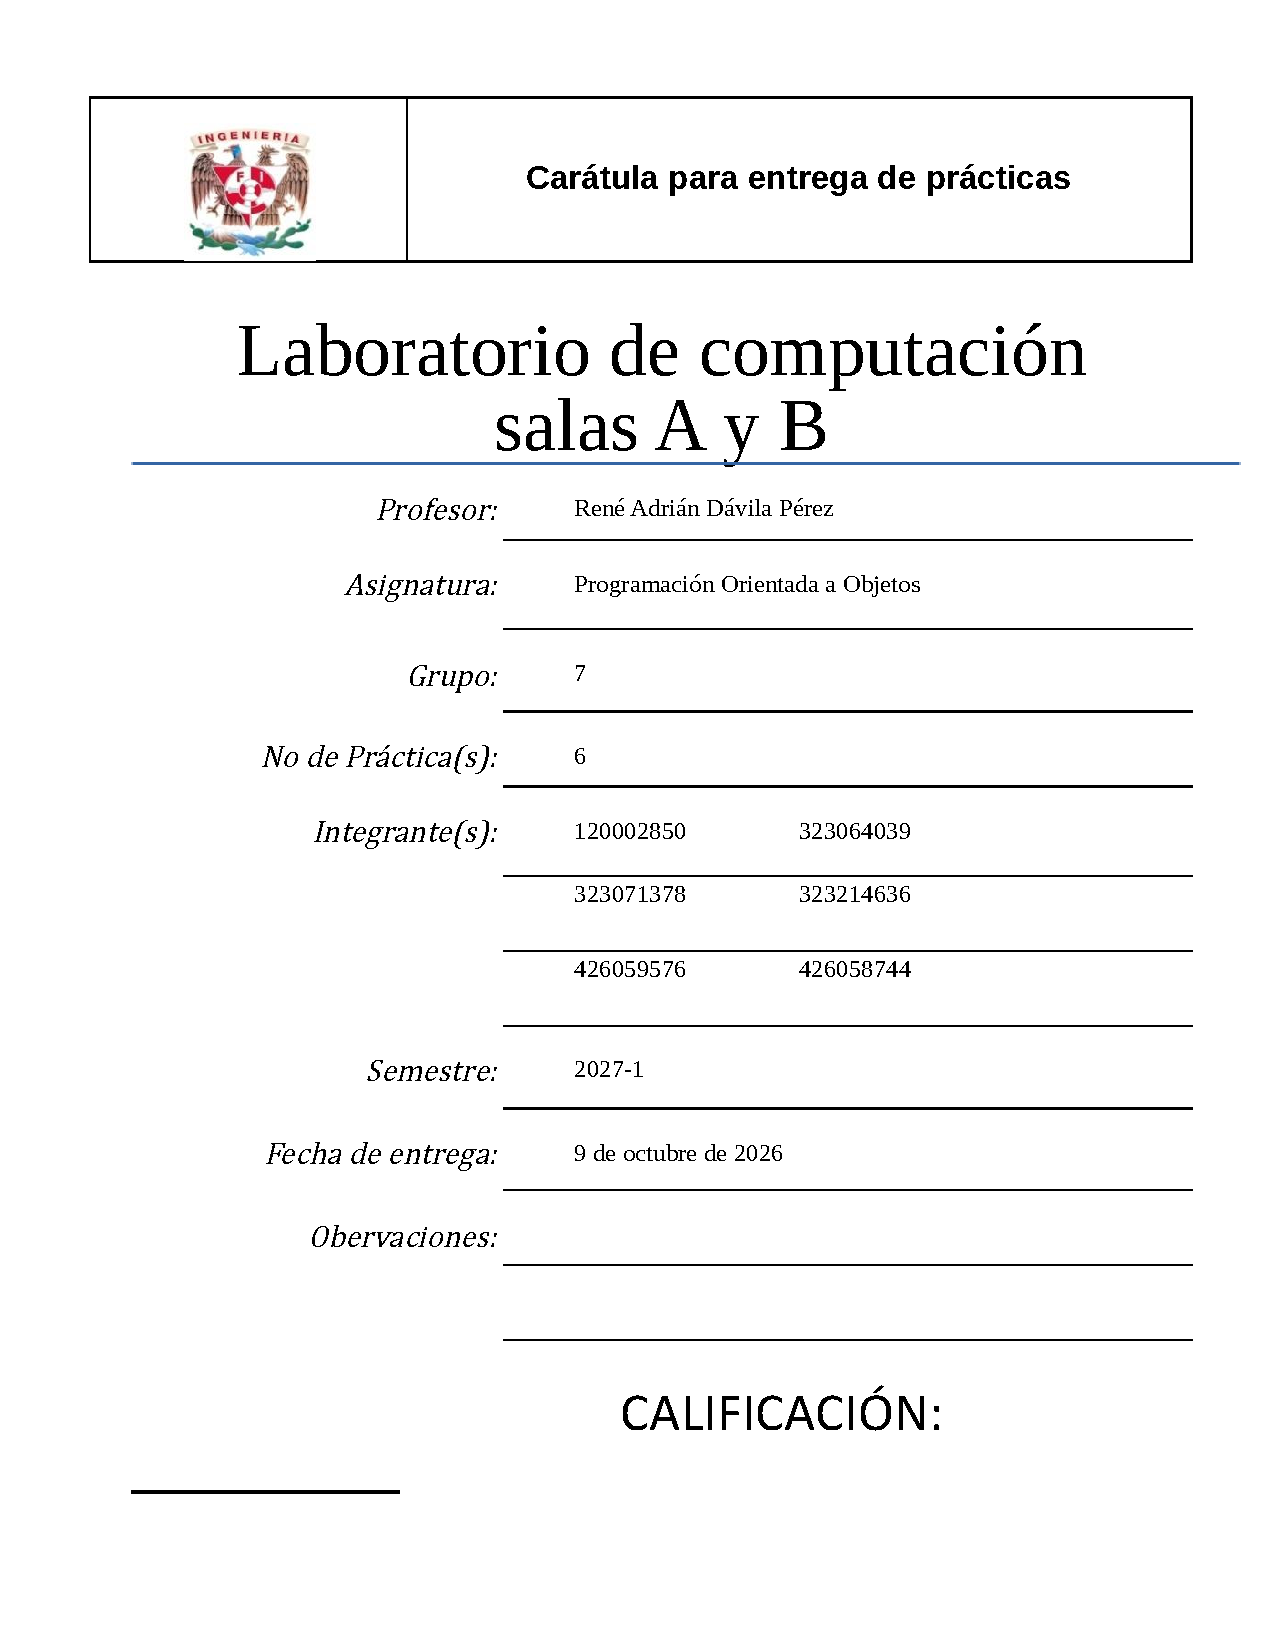
\includepdf[pages=1,pagecommand={}]{caratula.pdf}
\tableofcontents
\clearpage

\section{Introducci\'on}

\subsection{Planteamiento del problema}
En el curso de programaci\'on orientada a objetos se acumularon cinco pr\'acticas y un primer avance del proyecto hospitalario con decenas de clases dispersas en distintos estilos de organizaci\'on. Sin un esquema com\'un de paquetes resulta dif\'icil distribuir los programas, evitar colisiones de nombres y reutilizar los binarios en diferentes equipos. Adem\'as, la ausencia de documentaci\'on uniforme limita la comprensi\'on de cada m\'odulo. Esta pr\'actica aborda el problema mediante la recopilaci\'on de todas las entregas bajo la jerarqu\'ia institucional, la compilaci\'on y ejecuci\'on de archivos empaquetados y la generaci\'on de archivos JAR ejecutables con su documentaci\'on correspondiente.

\subsection{Motivaci\'on}
La industria del software distribuye componentes como unidades portables y autodocumentadas para reducir errores de integraci\'on y facilitar el mantenimiento \cite{deitel}. El uso de paquetes con dominio inverso garantiza trazabilidad acad\'emica y separa espacios de nombres por pr\'actica y proyecto \cite{oracle}. El empaquetado en un \'unico archivo con manifiesto ejecutable simplifica el despliegue sin manipular clases sueltas, mientras que la documentaci\'on generada con la herramienta oficial convierte comentarios estructurados en manuales navegables \cite{joyanes}. Reunir las cinco pr\'acticas y el proyecto en un recopilatorio homog\'eneo permite verificar que la compilaci\'on, la ejecuci\'on por classpath y la ejecuci\'on por JAR producen el mismo comportamiento.

\subsection{Objetivos}
El objetivo principal consiste en recopilar las cinco pr\'acticas y el primer avance del proyecto bajo la jerarqu\'ia \texttt{mx.unam.fi.die.poo.g7}, organizar la estructura com\'un de directorios y demostrar con el ejemplo base del sistema hospitalario c\'omo se compilan los archivos empaquetados, c\'omo se ejecutan por classpath, c\'omo se crea un JAR y c\'omo se ejecuta. De forma complementaria se documenta cada clase con Javadoc independiente, se estandarizan los diagramas UML y de flujo de todas las clases y se verifica el JAR del hospital con entradas deterministas.

\section{Marco Te\'orico}

\subsection{Archivos JAR y portabilidad}
Un archivo JAR es un contenedor basado en ZIP que agrupa clases compiladas, recursos y metadatos en una sola unidad transportable \cite{oracle}. El manifiesto \texttt{MANIFEST.MF} con la directiva \texttt{Main-Class} indica la clase de entrada para la ejecuci\'on directa. Esta t\'ecnica preserva la jerarqu\'ia de paquetes, reduce transferencias y evita p\'erdidas de archivos sueltos.

\subsection{Documentaci\'on con Javadoc}
Javadoc transforma comentarios \texttt{/** ... */} en p\'aginas HTML navegables \cite{joyanes}. Cada clase, atributo, constructor y m\'etodo se describe en lenguaje natural con \texttt{@param} para argumentos, \texttt{@return} para resultados y \texttt{@throws} para excepciones reales. La generaci\'on determinista desde consola con codificaci\'on UTF-8 y classpath controlado produce manuales reproducibles por clase sin enlaces entre clases.

\subsection{Paquetes y estructura de directorios}
Los paquetes con dominio inverso en min\'usculas evitan hom\'onimos y delimitan m\'odulos \cite{deitel}. El prefijo \texttt{mx.unam.fi.die.poo.g7} identifica a la Facultad de Ingenier\'ia y se subdivide en \texttt{p1} a \texttt{p5} y \texttt{proyecto}. La disposici\'on ubica fuentes en \texttt{src/}, binarios en \texttt{test/}, el ejecutable en \texttt{lib/} y la documentaci\'on en \texttt{doc/}, lo que separa editables de productos y facilita el versionado.

\subsection{Comandos b\'asicos para crear y correr un JAR en consola}
En Windows (\texttt{cmd}) y en Linux la herramienta \texttt{jar} del JDK crea y lista archives con sintaxis equivalente. Para crear un JAR con manifiesto ejecutable se emplea \texttt{jar cfm lib/SistemaHospitalario.jar MANIFEST.MF -C test mx/unam/fi/die/poo/g7/proyecto}, donde \texttt{c} crea, \texttt{f} indica archivo, \texttt{m} incorpora manifiesto y \texttt{-C} cambia al directorio de clases para preservar la jerarqu\'ia. El contenido se verifica con \texttt{jar tf lib/SistemaHospitalario.jar}, que lista entradas y manifiesto. La ejecuci\'on directa usa \texttt{java -jar lib/SistemaHospitalario.jar}, que localiza \texttt{Main-Class} sin declarar classpath. Para ejecutar una clase concreta sin manifiesto se usa \texttt{java -cp lib/SistemaHospitalario.jar mx.unam.fi.die.poo.g7.proyecto.Main}. En \texttt{cmd} las rutas usan diagonal invertida y las variables de entorno se ajustan con \texttt{set}, pero los subcomandos de \texttt{jar} y \texttt{java} conservan el mismo orden.

\subsection{C\'omo se compilan y c\'omo se corren los archivos Java empaquetados}
Un archivo con declaraci\'on \texttt{package} debe compilarse con destino expl\'icito para reproducir la jerarqu\'ia: \texttt{javac -encoding UTF-8 -parameters -d test src/mx/unam/fi/die/poo/g7/proyecto/*.java} genera \texttt{test/mx/.../*.class} con la codificaci\'on y los metadatos de par\'ametros requeridos. La compilaci\'on no produce ejecutable, solo bytecode verificable por la m\'aquina virtual. La ejecuci\'on por classpath indica d\'onde buscar clases: \texttt{java -cp test mx.unam.fi.die.poo.g7.proyecto.Main} resuelve el nombre totalmente calificado contra \texttt{test} y arranca el m\'etodo de entrada con la entrada est\'andar como \'unica fuente determinista. Cuando las clases ya est\'an empaquetadas, el classpath puede ser el JAR o el JAR puede autoarrancar con \texttt{-jar} si el manifiesto declara la clase principal. Ambos modos deben producir la misma salida ante la misma entrada, lo que demuestra portabilidad del empaquetado.

\section{Desarrollo}

\subsection{Investigaci\'on con inteligencia artificial}
Se formul\'o una consulta com\'un de 90 palabras conservada en \texttt{doc/Capturas/query.txt} sobre mejores pr\'acticas de JAR, generaci\'on de Javadoc y estructura \texttt{src}, \texttt{test} y \texttt{doc}. Cada integrante la plante\'o a un modelo de lenguaje para recabar criterios profesionales.

En la figura~\ref{fig:invalan} se reserva la evidencia de Alan.
\figura{../Capturas/1.png}{Consulta de investigaci\'on sobre JAR y Javadoc por Alan.}{fig:invalan}
En la figura~\ref{fig:invzoe} se reserva la evidencia de Zo\'e.
\figura{../Capturas/2.png}{Consulta de investigaci\'on sobre JAR y Javadoc por Zo\'e.}{fig:invzoe}
En la figura~\ref{fig:invluis} se reserva la evidencia de Luis.
\figura{../Capturas/3.png}{Consulta de investigaci\'on sobre JAR y Javadoc por Luis.}{fig:invluis}
En la figura~\ref{fig:invjoseph} se reserva la evidencia de Joseph.
\figura{../Capturas/4.png}{Consulta de investigaci\'on sobre JAR y Javadoc por Joseph.}{fig:invjoseph}
En la figura~\ref{fig:invhanniel} se reserva la evidencia de Hanniel.
\figura{../Capturas/5.png}{Consulta de investigaci\'on sobre JAR y Javadoc por Hanniel.}{fig:invhanniel}
En la figura~\ref{fig:invalex} se reserva la evidencia de Alex.
\figura{../Capturas/6.png}{Consulta de investigaci\'on sobre JAR y Javadoc por Alex.}{fig:invalex}

La s\'intesis confirma que la mejor manera de generar Javadoc es invocar la herramienta oficial desde consola con UTF-8 en entrada, salida y charset, con classpath compilado y sourcepath vac\'io, una clase por invocaci\'on y salida aislada por clase. El JAR debe contener solo clases verificadas con manifiesto preciso. La estructura homog\'enea separa fuentes, binarios, biblioteca y documentaci\'on para garantizar mantenibilidad y portabilidad.

\subsection{Organizaci\'on recopilatoria por paquetes}
Se reunieron las entregas sin crear c\'odigo nuevo, solo copi\'andolas bajo la jerarqu\'ia institucional:
\begin{itemize}
    \item \texttt{mx.unam.fi.die.poo.g7.p1}: calculadora b\'asica con siete operaciones y editor gr\'afico con figuras, lienzo y ventana.
    \item \texttt{mx.unam.fi.die.poo.g7.p2}: conteo de aprobados, mayor de diez n\'umeros y tabla de m\'ultiplos.
    \item \texttt{mx.unam.fi.die.poo.g7.p3}: lectura validada de entero de cinco d\'igitos y verificaci\'on de pal\'indromo.
    \item \texttt{mx.unam.fi.die.poo.g7.p4}: an\'alisis de frecuencias de palabras con colecciones y programa coordinador.
    \item \texttt{mx.unam.fi.die.poo.g7.p5}: entidades empleado y fecha con encapsulamiento y programas de ejemplo.
    \item \texttt{mx.unam.fi.die.poo.g7.proyecto}: sistema hospitalario con m\'edico, enfermero, paciente, contenedor y men\'u principal.
\end{itemize}
Cada m\'odulo conserva su l\'ogica original y solo se a\~nadieron comentarios Javadoc y constructores expl\'icitos donde faltaban para documentar el impl\'icito. La colisi\'on de nombre simple entre las dos clases \texttt{Main} de \texttt{p4} y \texttt{proyecto} se resolvi\'o organizando Javadoc, diagramas y pseudoc\'odigos por carpetas de origen (\texttt{P4/} y \texttt{Proyecto/}), sin renombrar clases ni inventar sufijos en el c\'odigo. Las relaciones se explican por paquetes: \texttt{AnalizadorPalabras} es usado por \texttt{Main} de \texttt{p4}; \texttt{Empleado} y \texttt{Fecha} son usados por sus programas principales; \texttt{Sistema} contiene listas de \texttt{Medico}, \texttt{Enfermero} y \texttt{Paciente}; el editor relaciona \texttt{Figura}, \texttt{CanvasPanel} y \texttt{EditorFrame} por composici\'on y uso del contexto gr\'afico.

\subsection{Diagramas UML y de flujo estandarizados}
Por cada clase se gener\'o un UML en tabla blanca con nombre, atributos tipados con visibilidad y operaciones con par\'ametros nombrados y retorno, con constructores expl\'icitos e impl\'icitos documentados, est\'aticos subrayados y finales con \texttt{\{readOnly\}}. Por cada clase se gener\'o un flujo de la operaci\'on relevante con estilos uniformes, decisiones binarias S\'i/No y ramas etiquetadas. Los pseudoc\'odigos reproducen la misma operaci\'on con pasos, condiciones y ciclos legibles.

\subsection{Recopilatorio por clase}

\subsubsection{Suma de P1 (Calculadora y operaciones basicas)}
Lee dos enteros y muestra la suma. El UML resume atributos y operaciones verificados contra la compilaci\'on y el flujo detalla la decisi\'on principal de la operaci\'on.

En la figura~\ref{fig:p1sumauml} se muestra el UML de \texttt{Suma} y en la figura~\ref{fig:p1sumaflujo} su flujo.
\figura{../Diagramas/P1/Suma_uml.png}{Diagrama UML de Suma (P1).}{fig:p1sumauml}
\figura{../Diagramas/P1/Suma_flujo.png}{Diagrama de flujo de Suma (P1).}{fig:p1sumaflujo}
\subsubsection{Resta de P1 (Calculadora y operaciones basicas)}
Lee dos enteros y opcion y muestra la resta. El UML resume atributos y operaciones verificados contra la compilaci\'on y el flujo detalla la decisi\'on principal de la operaci\'on.

En la figura~\ref{fig:p1restauml} se muestra el UML de \texttt{Resta} y en la figura~\ref{fig:p1restaflujo} su flujo.
\figura{../Diagramas/P1/Resta_uml.png}{Diagrama UML de Resta (P1).}{fig:p1restauml}
\figura{../Diagramas/P1/Resta_flujo.png}{Diagrama de flujo de Resta (P1).}{fig:p1restaflujo}
\subsubsection{Multiplicacion de P1 (Calculadora y operaciones basicas)}
Lee dos enteros y muestra el producto. El UML resume atributos y operaciones verificados contra la compilaci\'on y el flujo detalla la decisi\'on principal de la operaci\'on.

En la figura~\ref{fig:p1multiplicacionuml} se muestra el UML de \texttt{Multiplicacion} y en la figura~\ref{fig:p1multiplicacionflujo} su flujo.
\figura{../Diagramas/P1/Multiplicacion_uml.png}{Diagrama UML de Multiplicacion (P1).}{fig:p1multiplicacionuml}
\figura{../Diagramas/P1/Multiplicacion_flujo.png}{Diagrama de flujo de Multiplicacion (P1).}{fig:p1multiplicacionflujo}
\subsubsection{Division de P1 (Calculadora y operaciones basicas)}
Divide dos decimales con control de cero. El UML resume atributos y operaciones verificados contra la compilaci\'on y el flujo detalla la decisi\'on principal de la operaci\'on.

En la figura~\ref{fig:p1divisionuml} se muestra el UML de \texttt{Division} y en la figura~\ref{fig:p1divisionflujo} su flujo.
\figura{../Diagramas/P1/Division_uml.png}{Diagrama UML de Division (P1).}{fig:p1divisionuml}
\figura{../Diagramas/P1/Division_flujo.png}{Diagrama de flujo de Division (P1).}{fig:p1divisionflujo}
\subsubsection{Exponente de P1 (Calculadora y operaciones basicas)}
Calcula potencia con ciclo. El UML resume atributos y operaciones verificados contra la compilaci\'on y el flujo detalla la decisi\'on principal de la operaci\'on.

En la figura~\ref{fig:p1exponenteuml} se muestra el UML de \texttt{Exponente} y en la figura~\ref{fig:p1exponenteflujo} su flujo.
\figura{../Diagramas/P1/Exponente_uml.png}{Diagrama UML de Exponente (P1).}{fig:p1exponenteuml}
\figura{../Diagramas/P1/Exponente_flujo.png}{Diagrama de flujo de Exponente (P1).}{fig:p1exponenteflujo}
\subsubsection{Raiz de P1 (Calculadora y operaciones basicas)}
Calcula raiz con control de casos. El UML resume atributos y operaciones verificados contra la compilaci\'on y el flujo detalla la decisi\'on principal de la operaci\'on.

En la figura~\ref{fig:p1raizuml} se muestra el UML de \texttt{Raiz} y en la figura~\ref{fig:p1raizflujo} su flujo.
\figura{../Diagramas/P1/Raiz_uml.png}{Diagrama UML de Raiz (P1).}{fig:p1raizuml}
\figura{../Diagramas/P1/Raiz_flujo.png}{Diagrama de flujo de Raiz (P1).}{fig:p1raizflujo}
\subsubsection{Calculadora de P1 (Calculadora y operaciones basicas)}
Menu con siete operaciones. El UML resume atributos y operaciones verificados contra la compilaci\'on y el flujo detalla la decisi\'on principal de la operaci\'on.

En la figura~\ref{fig:p1calculadorauml} se muestra el UML de \texttt{Calculadora} y en la figura~\ref{fig:p1calculadoraflujo} su flujo.
\figura{../Diagramas/P1/Calculadora_uml.png}{Diagrama UML de Calculadora (P1).}{fig:p1calculadorauml}
\figura{../Diagramas/P1/Calculadora_flujo.png}{Diagrama de flujo de Calculadora (P1).}{fig:p1calculadoraflujo}
\subsubsection{Figura de P1 (Editor grafico de figuras)}
Registro inmutable de figura geometrica. El UML resume atributos y operaciones verificados contra la compilaci\'on y el flujo detalla la decisi\'on principal de la operaci\'on.

En la figura~\ref{fig:p1figurauml} se muestra el UML de \texttt{Figura} y en la figura~\ref{fig:p1figuraflujo} su flujo.
\figura{../Diagramas/P1/Figura_uml.png}{Diagrama UML de Figura (P1).}{fig:p1figurauml}
\figura{../Diagramas/P1/Figura_flujo.png}{Diagrama de flujo de Figura (P1).}{fig:p1figuraflujo}
\subsubsection{CanvasPanel de P1 (Editor grafico de figuras)}
Panel de dibujo con deshacer y exportacion. El UML resume atributos y operaciones verificados contra la compilaci\'on y el flujo detalla la decisi\'on principal de la operaci\'on.

En la figura~\ref{fig:p1canvaspaneluml} se muestra el UML de \texttt{CanvasPanel} y en la figura~\ref{fig:p1canvaspanelflujo} su flujo.
\figura{../Diagramas/P1/CanvasPanel_uml.png}{Diagrama UML de CanvasPanel (P1).}{fig:p1canvaspaneluml}
\figura{../Diagramas/P1/CanvasPanel_flujo.png}{Diagrama de flujo de CanvasPanel (P1).}{fig:p1canvaspanelflujo}
\subsubsection{EditorFrame de P1 (Editor grafico de figuras)}
Ventana principal del editor. El UML resume atributos y operaciones verificados contra la compilaci\'on y el flujo detalla la decisi\'on principal de la operaci\'on.

En la figura~\ref{fig:p1editorframeuml} se muestra el UML de \texttt{EditorFrame} y en la figura~\ref{fig:p1editorframeflujo} su flujo.
\figura{../Diagramas/P1/EditorFrame_uml.png}{Diagrama UML de EditorFrame (P1).}{fig:p1editorframeuml}
\figura{../Diagramas/P1/EditorFrame_flujo.png}{Diagrama de flujo de EditorFrame (P1).}{fig:p1editorframeflujo}
\subsubsection{Ejercicio1\_P2 de P2 (Estructuras de control y tablas)}
Cuenta aprobados y reprobados. El UML resume atributos y operaciones verificados contra la compilaci\'on y el flujo detalla la decisi\'on principal de la operaci\'on.

En la figura~\ref{fig:p2ejercicio1p2uml} se muestra el UML de \texttt{Ejercicio1\_P2} y en la figura~\ref{fig:p2ejercicio1p2flujo} su flujo.
\figura{../Diagramas/P2/Ejercicio1_P2_uml.png}{Diagrama UML de Ejercicio1\_P2 (P2).}{fig:p2ejercicio1p2uml}
\figura{../Diagramas/P2/Ejercicio1_P2_flujo.png}{Diagrama de flujo de Ejercicio1\_P2 (P2).}{fig:p2ejercicio1p2flujo}
\subsubsection{Ejercicio2\_P2 de P2 (Estructuras de control y tablas)}
Determina el mayor de diez numeros. El UML resume atributos y operaciones verificados contra la compilaci\'on y el flujo detalla la decisi\'on principal de la operaci\'on.

En la figura~\ref{fig:p2ejercicio2p2uml} se muestra el UML de \texttt{Ejercicio2\_P2} y en la figura~\ref{fig:p2ejercicio2p2flujo} su flujo.
\figura{../Diagramas/P2/Ejercicio2_P2_uml.png}{Diagrama UML de Ejercicio2\_P2 (P2).}{fig:p2ejercicio2p2uml}
\figura{../Diagramas/P2/Ejercicio2_P2_flujo.png}{Diagrama de flujo de Ejercicio2\_P2 (P2).}{fig:p2ejercicio2p2flujo}
\subsubsection{Ejercicio3\_P2 de P2 (Estructuras de control y tablas)}
Imprime tabla de multiplos. El UML resume atributos y operaciones verificados contra la compilaci\'on y el flujo detalla la decisi\'on principal de la operaci\'on.

En la figura~\ref{fig:p2ejercicio3p2uml} se muestra el UML de \texttt{Ejercicio3\_P2} y en la figura~\ref{fig:p2ejercicio3p2flujo} su flujo.
\figura{../Diagramas/P2/Ejercicio3_P2_uml.png}{Diagrama UML de Ejercicio3\_P2 (P2).}{fig:p2ejercicio3p2uml}
\figura{../Diagramas/P2/Ejercicio3_P2_flujo.png}{Diagrama de flujo de Ejercicio3\_P2 (P2).}{fig:p2ejercicio3p2flujo}
\subsubsection{Palindromo de P3 (Palindromos y colecciones)}
Verifica palindromo de cinco digitos. El UML resume atributos y operaciones verificados contra la compilaci\'on y el flujo detalla la decisi\'on principal de la operaci\'on.

En la figura~\ref{fig:p3palindromouml} se muestra el UML de \texttt{Palindromo} y en la figura~\ref{fig:p3palindromoflujo} su flujo.
\figura{../Diagramas/P3/Palindromo_uml.png}{Diagrama UML de Palindromo (P3).}{fig:p3palindromouml}
\figura{../Diagramas/P3/Palindromo_flujo.png}{Diagrama de flujo de Palindromo (P3).}{fig:p3palindromoflujo}
\subsubsection{AnalizadorPalabras de P4 (Analisis de palabras)}
Cuenta frecuencias con colecciones. El UML resume atributos y operaciones verificados contra la compilaci\'on y el flujo detalla la decisi\'on principal de la operaci\'on.

En la figura~\ref{fig:p4analizadorpalabrasuml} se muestra el UML de \texttt{AnalizadorPalabras} y en la figura~\ref{fig:p4analizadorpalabrasflujo} su flujo.
\figura{../Diagramas/P4/AnalizadorPalabras_uml.png}{Diagrama UML de AnalizadorPalabras (P4).}{fig:p4analizadorpalabrasuml}
\figura{../Diagramas/P4/AnalizadorPalabras_flujo.png}{Diagrama de flujo de AnalizadorPalabras (P4).}{fig:p4analizadorpalabrasflujo}
\subsubsection{Main de P4 (Analisis de palabras)}
Coordina lectura y muestra duplicadas. El UML resume atributos y operaciones verificados contra la compilaci\'on y el flujo detalla la decisi\'on principal de la operaci\'on.

En la figura~\ref{fig:p4mainuml} se muestra el UML de \texttt{Main} y en la figura~\ref{fig:p4mainflujo} su flujo.
\figura{../Diagramas/P4/Main_uml.png}{Diagrama UML de Main (P4).}{fig:p4mainuml}
\figura{../Diagramas/P4/Main_flujo.png}{Diagrama de flujo de Main (P4).}{fig:p4mainflujo}
\subsubsection{Empleado de P5 (Encapsulamiento empleado y fecha)}
Entidad empleado con salario validado. El UML resume atributos y operaciones verificados contra la compilaci\'on y el flujo detalla la decisi\'on principal de la operaci\'on.

En la figura~\ref{fig:p5empleadouml} se muestra el UML de \texttt{Empleado} y en la figura~\ref{fig:p5empleadoflujo} su flujo.
\figura{../Diagramas/P5/Empleado_uml.png}{Diagrama UML de Empleado (P5).}{fig:p5empleadouml}
\figura{../Diagramas/P5/Empleado_flujo.png}{Diagrama de flujo de Empleado (P5).}{fig:p5empleadoflujo}
\subsubsection{Fecha de P5 (Encapsulamiento empleado y fecha)}
Entidad fecha con dia mes y anio. El UML resume atributos y operaciones verificados contra la compilaci\'on y el flujo detalla la decisi\'on principal de la operaci\'on.

En la figura~\ref{fig:p5fechauml} se muestra el UML de \texttt{Fecha} y en la figura~\ref{fig:p5fechaflujo} su flujo.
\figura{../Diagramas/P5/Fecha_uml.png}{Diagrama UML de Fecha (P5).}{fig:p5fechauml}
\figura{../Diagramas/P5/Fecha_flujo.png}{Diagrama de flujo de Fecha (P5).}{fig:p5fechaflujo}
\subsubsection{MainEmpleado de P5 (Encapsulamiento empleado y fecha)}
Crea empleados y calcula anual. El UML resume atributos y operaciones verificados contra la compilaci\'on y el flujo detalla la decisi\'on principal de la operaci\'on.

En la figura~\ref{fig:p5mainempleadouml} se muestra el UML de \texttt{MainEmpleado} y en la figura~\ref{fig:p5mainempleadoflujo} su flujo.
\figura{../Diagramas/P5/MainEmpleado_uml.png}{Diagrama UML de MainEmpleado (P5).}{fig:p5mainempleadouml}
\figura{../Diagramas/P5/MainEmpleado_flujo.png}{Diagrama de flujo de MainEmpleado (P5).}{fig:p5mainempleadoflujo}
\subsubsection{MainFecha de P5 (Encapsulamiento empleado y fecha)}
Crea fecha y la muestra. El UML resume atributos y operaciones verificados contra la compilaci\'on y el flujo detalla la decisi\'on principal de la operaci\'on.

En la figura~\ref{fig:p5mainfechauml} se muestra el UML de \texttt{MainFecha} y en la figura~\ref{fig:p5mainfechaflujo} su flujo.
\figura{../Diagramas/P5/MainFecha_uml.png}{Diagrama UML de MainFecha (P5).}{fig:p5mainfechauml}
\figura{../Diagramas/P5/MainFecha_flujo.png}{Diagrama de flujo de MainFecha (P5).}{fig:p5mainfechaflujo}
\subsubsection{Medico de Proyecto (Sistema hospitalario)}
Medico con especialidad y pacientes. El UML resume atributos y operaciones verificados contra la compilaci\'on y el flujo detalla la decisi\'on principal de la operaci\'on.

En la figura~\ref{fig:proyectomedicouml} se muestra el UML de \texttt{Medico} y en la figura~\ref{fig:proyectomedicoflujo} su flujo.
\figura{../Diagramas/Proyecto/Medico_uml.png}{Diagrama UML de Medico (Proyecto).}{fig:proyectomedicouml}
\figura{../Diagramas/Proyecto/Medico_flujo.png}{Diagrama de flujo de Medico (Proyecto).}{fig:proyectomedicoflujo}
\subsubsection{Enfermero de Proyecto (Sistema hospitalario)}
Enfermero con atencion por especialidad. El UML resume atributos y operaciones verificados contra la compilaci\'on y el flujo detalla la decisi\'on principal de la operaci\'on.

En la figura~\ref{fig:proyectoenfermerouml} se muestra el UML de \texttt{Enfermero} y en la figura~\ref{fig:proyectoenfermeroflujo} su flujo.
\figura{../Diagramas/Proyecto/Enfermero_uml.png}{Diagrama UML de Enfermero (Proyecto).}{fig:proyectoenfermerouml}
\figura{../Diagramas/Proyecto/Enfermero_flujo.png}{Diagrama de flujo de Enfermero (Proyecto).}{fig:proyectoenfermeroflujo}
\subsubsection{Paciente de Proyecto (Sistema hospitalario)}
Paciente con estado y asignaciones. El UML resume atributos y operaciones verificados contra la compilaci\'on y el flujo detalla la decisi\'on principal de la operaci\'on.

En la figura~\ref{fig:proyectopacienteuml} se muestra el UML de \texttt{Paciente} y en la figura~\ref{fig:proyectopacienteflujo} su flujo.
\figura{../Diagramas/Proyecto/Paciente_uml.png}{Diagrama UML de Paciente (Proyecto).}{fig:proyectopacienteuml}
\figura{../Diagramas/Proyecto/Paciente_flujo.png}{Diagrama de flujo de Paciente (Proyecto).}{fig:proyectopacienteflujo}
\subsubsection{Sistema de Proyecto (Sistema hospitalario)}
Contenedor que registra personal y pacientes. El UML resume atributos y operaciones verificados contra la compilaci\'on y el flujo detalla la decisi\'on principal de la operaci\'on.

En la figura~\ref{fig:proyectosistemauml} se muestra el UML de \texttt{Sistema} y en la figura~\ref{fig:proyectosistemaflujo} su flujo.
\figura{../Diagramas/Proyecto/Sistema_uml.png}{Diagrama UML de Sistema (Proyecto).}{fig:proyectosistemauml}
\figura{../Diagramas/Proyecto/Sistema_flujo.png}{Diagrama de flujo de Sistema (Proyecto).}{fig:proyectosistemaflujo}
\subsubsection{Main de Proyecto (Sistema hospitalario)}
Menu principal del hospital. El UML resume atributos y operaciones verificados contra la compilaci\'on y el flujo detalla la decisi\'on principal de la operaci\'on.

En la figura~\ref{fig:proyectomainuml} se muestra el UML de \texttt{Main} y en la figura~\ref{fig:proyectomainflujo} su flujo.
\figura{../Diagramas/Proyecto/Main_uml.png}{Diagrama UML de Main (Proyecto).}{fig:proyectomainuml}
\figura{../Diagramas/Proyecto/Main_flujo.png}{Diagrama de flujo de Main (Proyecto).}{fig:proyectomainflujo}

\section{Resultados}

\subsection{Compilaci\'on de archivos empaquetados}
Como entrada se tomaron los cinco archivos del paquete \texttt{mx.unam.fi.die.poo.g7.proyecto} ubicados en \texttt{src/}. El resultado esperado calculado consist\'ia en la generaci\'on sin errores de la jerarqu\'ia \texttt{test/mx/.../proyecto/*.class} con codificaci\'on UTF-8. El resultado observado ejecutado coincidi\'o: la invocaci\'on termin\'o sin salida de error y list\'o los binarios. En la figura~\ref{fig:compilacionproyecto} se muestra la captura real de la compilaci\'on.
\figura{../Capturas/compilacion_proyecto.png}{Compilaci\'on real de los archivos empaquetados del proyecto.}{fig:compilacionproyecto}
\subsection{Ejecuci\'on por classpath}
Como entrada determinista se suministr\'o por la entrada est\'andar la secuencia \texttt{1}, \texttt{10} y \texttt{0}: cargar datos demo, ver especialidades y salir. El resultado esperado calculado era el despliegue del men\'u, la confirmaci\'on de tres especialidades, tres m\'edicos, tres enfermeros y tres pacientes, el listado de cardiolog\'ia, pediatr\'ia y traumatolog\'ia y el mensaje de salida. El resultado observado ejecutado con \texttt{java -cp test mx.unam.fi.die.poo.g7.proyecto.Main} coincidi\'o de forma exacta. En la figura~\ref{fig:ejecucioncpproyecto} se muestra la captura real.
\figura{../Capturas/ejecucion_cp_proyecto.png}{Ejecuci\'on real por classpath del sistema hospitalario.}{fig:ejecucioncpproyecto}
\subsection{Creaci\'on del JAR y verificaci\'on de contenido}
Como entrada se usaron los binarios verificados de \texttt{test} y el manifiesto con \texttt{Main-Class: mx.unam.fi.die.poo.g7.proyecto.Main}. El resultado esperado calculado era un \'unico archivo \texttt{lib/SistemaHospitalario.jar} con seis entradas de clases m\'as manifiesto. El resultado observado con \texttt{jar cfm} y \texttt{jar tf} confirm\'o el contenido. En la figura~\ref{fig:creacionjarproyecto} se muestra la captura real.
\figura{../Capturas/creacion_jar_proyecto.png}{Creaci\'on real del JAR y listado de su contenido.}{fig:creacionjarproyecto}
\subsection{Ejecuci\'on del JAR}
Como entrada se suministr\'o \texttt{1}, \texttt{11} y \texttt{0}: demo, ver m\'edicos y salir. El resultado esperado era id\'entico al de classpath pero invocando \texttt{java -jar lib/SistemaHospitalario.jar} sin declarar classpath. El resultado observado coincidi\'o, con el listado de m\'edicos y pacientes a cargo. En la figura~\ref{fig:ejecucionjarproyecto} se muestra la captura real.
\figura{../Capturas/ejecucion_jar_proyecto.png}{Ejecuci\'on real del JAR del sistema hospitalario.}{fig:ejecucionjarproyecto}
La generaci\'on de Javadoc independiente por clase finaliz\'o sin errores ni advertencias en \texttt{doc/Javadoc/P1/}, \texttt{P2/}, \texttt{P3/}, \texttt{P4/}, \texttt{P5/} y \texttt{Proyecto/}, con una carpeta por clase y navegaci\'on local. El JAR \'unico en \texttt{lib/} contiene solo el proyecto verificado; \texttt{test/} conserva los 28 binarios del recopilatorio para classpath y documentaci\'on.

\section{Conclusiones}
La recopilaci\'on bajo paquetes institucionales elimin\'o la dispersi\'on de entregas y resolvi\'o colisiones aparentes como la de las dos clases \texttt{Main} mediante organizaci\'on por origen, sin alterar la l\'ogica original. La separaci\'on entre fuentes, binarios, biblioteca y documentaci\'on demostr\'o ser la base m\'inima para portabilidad y mantenimiento en equipos heterog\'eneos.

Los comandos de compilaci\'on con destino expl\'icito, ejecuci\'on por classpath y empaquetado con manifiesto forman una cadena reproducible: el mismo bytecode produce la misma salida ya sea desde \texttt{test} o desde el JAR. La documentaci\'on estandarizada y los diagramas uniformes permiten comparar clases de distinta dificultad con el mismo lenguaje visual y textual.

El ejemplo base del hospital valid\'o la robustez del flujo con entradas deterministas de demo y consulta, confirmando que un dise\~no defensivo con validaci\'on de rangos y colecciones ordenadas sostiene la escalabilidad del sistema sin c\'odigo adicional en esta pr\'actica.

\begin{thebibliography}{9}

\bibitem{deitel}
P.~J. Deitel y H.~M. Deitel,
\emph{C\'omo programar en Java},
10.\textsuperscript{a}~ed.,
Pearson Educaci\'on, M\'exico, 2016.

\bibitem{joyanes}
L.~Joyanes Aguilar,
\emph{Fundamentos de programaci\'on: algoritmos, estructuras de datos y objetos},
4.\textsuperscript{a}~ed.,
McGraw-Hill Interamericana, Madrid, 2008.

\bibitem{oracle}
Oracle Corporation,
\emph{The Java Tutorials: Packaging Programs in JAR Files},
Oracle Java SE Documentation, 2024.

\end{thebibliography}

\end{document}
